
% XXX- discuss GtkBin; which widgets have a window, which do not --image and label do not, and we mightwant them too,
%   modify_bg() only affects widgets that have an associated gtk.gdk.Window.
% > Widgets that do not have an associated window include .... gtk.Arrow,
% > gtk.Bin, gtk.Box, gtk.Button, gtk.CheckButton, gtk.Fixed , gtk.Image ,
% > gtk.Label , gtk.MenuItem , gtk.Notebook , gtk.Paned , gtk.RadioButton ,
% > gtk.Range , gtk.ScrolledWindow , gtk.Separator , gtk.Table , gtk.Toolbar ,
% > gtk.AspectFrame , gtk.Frame , gtk.VBox , gtk.HBox , gtk.VSeparator ,
% > gtk.HSeparator . These widgets can be added to a gtk.EventBox to overcome
% > this limitation.




%% RGtk2 chapter
\chapter{RGtk2: Overview}
%%\section{Introduction}
\label{sec:RGtk2-Introduction}
%% intorduction

%% Technical, but short beginning

As the name implies, the \pkg{RGtk2} package is an interface, or
binding, between \R\/ and \GTK, a mature, cross-platform GUI
toolkit. The letters \emph{GTK} stand for the \emph{GIMP ToolKit},
with the word \emph{GIMP} recording the origin of the library as part
of the GNU Image Manipulation Program. \pkg{GTK+} provides the same
widgets on every platform, though it can be customized to emulate
platform-specific look and feel. The library is written in
\proglang{C}, which facilitates access from languages like
\proglang{R} that are also implemented in \proglang{C}. \pkg{GTK+} is
licensed under the \textit{Lesser GNU Public License} (LGPL), while
\pkg{RGtk2} is under the \textit{GNU Public License} (GPL).
The package is available from the Comprehensive \proglang{R} Archive
Network (CRAN) at \url{http://CRAN.R-project.org/package=RGtk2}.

The name \pkg{RGtk2} also implies that there exists a package named
\pkg{RGtk}, which is indeed the case. The original \pkg{RGtk} is bound
to the previous generation of \pkg{GTK+}, version 1.2. \pkg{RGtk2} is
based on \pkg{GTK+ 2.0}, the current generation. This book covers
\pkg{RGtk2} specifically, although many of the fundamental features of
\pkg{RGtk2} are inherited from \pkg{RGtk}. 

\pkg{RGtk2} provides virtually all of the functionality in \GTK\/ to
the \R\/ programmer. In addition, \pkg{RGtk2} interfaces with several
other libraries in the \GTK\/ stack: Pango for font rendering; Cairo
for vector graphics; GdkPixbuf for image manipulation; libglade for
designing GUI layouts from an XML description; ATK for accessible
interfaces; and GDK, an abstraction over the native windowing system,
supporting either X11 or Windows. These libraries are multi-platform
and extensive and have been used for many major projects, such as the
Linux versions of Firefox and Open Office.

The API of each of these libraries is mapped to \R\/ in a way that is
consistent with \R\/ conventions and familiar to the \R\/
user. Much of the \pkg{RGtk2} API consists of autogenerated \R\/
functions that call into the one of the underlying libraries. For
example, the \R\/ function \function{gtkContainerAdd} eventually calls
the C function \code{gtk\_container\_add}. The naming convention is
that the C name has its underscores removed and each following letter
capitalized (camelback style).

The full API for \GTK\/ is quite large, and complete documentation of
it is beyond our scope. However, the \GTK\/ documentation is
algorithmically converted into the \R\/ help format during the
generation of \pkg{RGtk2}. This conveniently allows the programmer to
refer to the appropriate documentation within an \R\/ session, without
having to consult a web page, such as
\url{http://library.gnome.org/devel/gtk/stable/}, which lists the
\proglang{C} API of the stable versions \GTK.

In this chapter, we give an overview of how \pkg{RGtk2} maps the
\GTK\/ API, including its classes, constructors, methods, properties,
signals and enumerations, to an \R-level API that is relatively
familiar to and convenient for an \R\/ user. A simple GUI will be
gradually constructed to demonstrate the API.

%%% ------- OOP --------------

\section{Objects and Classes}

In any toolkit, all widget types have functionality in common. For
example, they are all drawn on the screen in a consistent style. They
can be hidden and shown again. To formalize this relationship and to
simplify implementation by sharing code between widgets, \pkg{GTK+},
like many other toolkits, defines an inheritance hierarchy for its
widget types. In the parlance of object-oriented programming, each
type is represented by a \textit{class}.

For specifying the hierarchy, \pkg{GTK+} relies on \pkg{GObject}, a
\proglang{C} library that implements a class-based, single-inheritance
object-oriented system. A \pkg{GObject} class encapsulates behaviors
that all instances of the class share. Every class has at most one
parent from which it inherits the behaviors of its ancestors. A
subclass can override some specific inherited behaviors. The interface
defined by a class consists of constructors, methods, properties,
and signals. 
% TODO: example of gTypeGetAncestors

Single inheritance can be restrictive when a class performs multiple
roles in a program. To circumvent this, \pkg{GTK+} adopts the popular
concept of the \textit{interface}, which is essentially a contract
that specifies which methods, properties and signals a class must
implement. As with languages like Java and \proglang{C\#}, a class can
\textit{implement} multiple interfaces, and an interface can be
composed of other interfaces. An interface allows the programmer to
treat all instances of implementing classes in a similar way. However,
unlike class inheritance, the implementation of the methods,
properties and signals is not shared.
% TODO: example of gTypeGetInterfaces

We explain the constructors, methods, properties and signals of
classes and interfaces in the following sections and demonstrate them
in the construction of a simple ``Hello World'' GUI, shown in
Figure~\ref{fig:hello-world}. A more detailed and technical
explanation of \pkg{GObject} is available in
Section~\ref{sec:gobject-primer}.

\begin{figure}[h!tbp]
  \begin{center}
    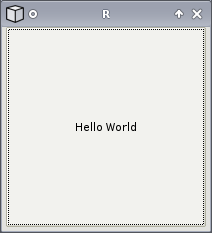
\includegraphics[width=2in]{hello-world.png}
    \caption{\label{fig:hello-world}``Hello World'' in GTK+. 
      A window containing a single button displaying a label with the text
      \code{Hello World}.}
  \end{center}
\end{figure}

\section{Constructors}

The first step in our example is to create a top-level window to
contain our GUI.  Creating an instance of a GTK\/ widget requires
calling a single \R\/ function, known as a constructor. Following \R\/
conventions, the constructor for a class has the same name as the
class, except the first character is lowercase. The following
statement constructs an instance of the \code{GtkWindow} class:
\begin{Schunk}
\begin{Sinput}
 window <- gtkWindow("toplevel", show = FALSE)
\end{Sinput}
\end{Schunk}
%
The first argument to the constructor for \code{GtkWindow} instructs
the window manager to treat the window as top-level.  The \code{show}
argument is the last argument for every widget constructor. It
indicates whether the widget should be made visible immediately after
construction.  The default value of \code{show} is \code{TRUE}. In
this case we want to defer showing the window until after we finish
constructing our simple GUI.

At the \GTK\/ level, a class usually has multiple constructors, each
implemented as a separate C function. In \pkg{RGtk2}, the names of
these functions all end with \code{New}. The ``meta'' constructor
\function{gtkWindow}, called above, automatically delegates to one of
the low-level constructors, based on the provided arguments.

A \GTK\/ object created by the \R\/ user has an \R-level object as its
proxy. Thus, \code{window} is a reference to a \class{GtkWindow}
instance.  The class hierarchy of a proxy object is represented by the
\code{class} attribute. One interprets the attribute according to S3
conventions, so that the class names are in order from most to least
derived:
\begin{Schunk}
\begin{Sinput}
 class(window)
\end{Sinput}
\begin{Soutput}
[1] "GtkWindow"         "GtkBin"            "GtkContainer"     
[4] "GtkWidget"         "GtkObject"         "GInitiallyUnowned"
[7] "GObject"           "RGtkObject"       
\end{Soutput}
\end{Schunk}
%
We find that the \class{GtkWindow} class inherits methods,
properties, and signals from the \class{GtkBin}, \class{GtkContainer},
\class{GtkWidget}, \class{GtkObject}, \class{GInitiallyUnowned}, and
\class{GObject} classes. Every type of \pkg{GTK+} widget inherits from
the base \code{GtkWidget} class, which implements the general
characteristics shared by all widget classes, e.g., properties storing
the location and background color; methods for hiding, showing and
painting the widget. We can also query \code{window} for the
interfaces it implements:
\begin{Schunk}
\begin{Sinput}
 interface.GObject(window)